\documentclass[a4paper,11pt,UTF8]{article}
\usepackage{ctex}
\usepackage{amsmath,amsthm,amssymb,amsfonts}
\usepackage{amsmath}
\usepackage[a4paper]{geometry}
\usepackage{graphicx}
\usepackage{microtype}
\usepackage{siunitx}
\usepackage{booktabs}
\usepackage[colorlinks=false, pdfborder={0 0 0}]{hyperref}
\usepackage{cleveref}
\usepackage{esint} 
\usepackage{graphicx}
\usepackage{ragged2e}
\usepackage{pifont}
\usepackage{extarrows}
\usepackage{mathptmx}
\usepackage{float}
\usepackage{caption}
\captionsetup[figure]{name={Figure}}
%opening
\title{数字电子技术作业(一)}
\author{谢悦晋 \quad U202210333}
\date{Sept 24th, 2023 }
\begin{document}
\maketitle
\noindent\textbf{2.1.3} 应用反演规则和对偶规则,求下列函数的非函数和对偶函数:\\
(1)$L=A\cdot B+\overline{A}\cdot\overline{B}$\\
(2)$L=\overline{A}\cdot\overline{B}+\overline{\overline{A}\cdot B\cdot\overline{C}}\cdot D$\\
解:\\
(1)$\overline{L}=(\overline{A}+\overline{B})(A+B), L^\prime=(A+B)(\overline{A}+\overline{B})$\\
(2)$\overline{L}=(A+B)(\overline{A+\overline{B}+C}+\overline{D}), L^\prime=(\overline{A}+\overline{B})(\overline{\overline{A}+B+\overline{C}}+D)$\\
\textbf{2.2.3} 试写出下列各个函数的最小项表达式:\\
(3)$L=\overline{\overline{AB}+ABD}(B+\overline{C}D)$\\
(4)$L=\overline{(A\overline{B}+B\overline{C})\overline{AB}}$\\
解:\\
(3)\\$\begin{aligned}
	L&=AB\cdot\overline{ABD}(B+\overline{C}D)\\
	&=AB\cdot(\overline{A}+\overline{B}+\overline{D})(B+\overline{C}D)\\
	&=AB\overline{D}(B+\overline{C}D)\\
	&=AB\overline{D}
\end{aligned}$\\
(4)\\$\begin{aligned}
	L&=\overline{(A\overline{B}+B\overline{C})}+AB\\
	&=\overline{A\overline{B}}\cdot\overline{B\overline{C}}+AB\\
	&=(\overline{A}+B)(\overline{B}+C)+AB\\
	&=B+\overline{A}C\\
	&=B(\overline{A}+A)(\overline{C}+C)\\
	&=ABC+\overline{A}B\overline{C}+\overline{A}BC+AB\overline{C}+\overline{A}BC
\end{aligned}$\\
\textbf{2.3.1}
用代数法将下列各式化简成最简的与-或表达式\\
(1)$\overline{\overline{(\overline{A}+B)}+\overline{(A+B)}+(\overline{\overline{A}B})(\overline{A\overline{B}})}\\$
(2)$\overline{B}+ABC+\overline{AC}+\overline{AB}$\\
(3)${ABC}{\overline{D}+ABD+BC}{\overline{D}+ABCD+B}{\overline{C}}$\\
(4)$\overline{{\overline{AC+\overline{A}BC}+\overline{B}C+AB\overline{C}}}$\\
解:\\
(1)\\
$\begin{aligned}
	L&=\overline{A\overline{B}+\overline{A}\cdot\overline{B}+(A+\overline{B})(\overline{A}+B)}\\
	&=\overline{\overline{B}+\overline{A}B+A\overline{B}}\\
	&=\overline{\overline{A}B+A\overline{B}}\\
	&=\overline{\overline{A}B}\cdot\overline{A\overline{B}}\\
	&=(A+\overline{B})(\overline{A}+B)\\
	&=\overline{A}B+A\overline{B}
\end{aligned}$\\
(2)\\
$\begin{aligned}
	L&=\overline{B}+A\overline{B}C+\overline{A}+\overline{C}+\overline{A}+\overline{B}\\
	&=\overline{A}+\overline{B}+\overline{C}+A\overline{B}C\\
	&=\overline{A}+\overline{B}C+\overline{B}+\overline{C}\\
	&=\overline{A}+\overline{B}+\overline{C}
\end{aligned}$\\
(3)\\
$\begin{aligned}
	L&=ABC+ABD+BC\overline{D}+B\overline{C}\\
	&=B\overline{C}+B\overline{D}+AB
\end{aligned}$\\
(4)\\
$\begin{aligned}
	L&=(AC+\overline{A}BC)\cdot\overline{\overline{B}C}\cdot\overline{AB\overline{C}}\\
	&=C(A+\overline{A}B)(B+\overline{C})(\overline{A}+\overline{B}+C)\\
	&=(A+B)BC(\overline{A}+\overline{B}+C)\\
	&=(ABC+BC)(\overline{A}+\overline{B}+C)\\
	&=ABC+\overline{A}BC+BC\\
	&=BC
\end{aligned}$\\
\textbf{2.4.3} 用卡诺图法化简下列各式:\\
(1)$A\overline{B}CD+AB\overline{C}D+A\overline{B}+A\overline{D}+A\overline{B}C$\\
(2)$A\overline{B}CD+D(\overline{B}\cdot\overline{C}D)+(A+C)B\overline{D}+\overline{A}\overline{(\overline{B}+C)}
$\\
(3)$
L(A,B,C,D)=\sum m(0,2,4,8,10,12)
$\\
(4)$
L(A,B,C,D)=\sum m(0,4,6,13,14,15)+\sum d(1,2,3,5,7,9,10,11)
$\\ 
解:\\
(1)卡诺图如下:(其中列为AB, 行为CD)
\begin{figure}[H] 
	\centering 
	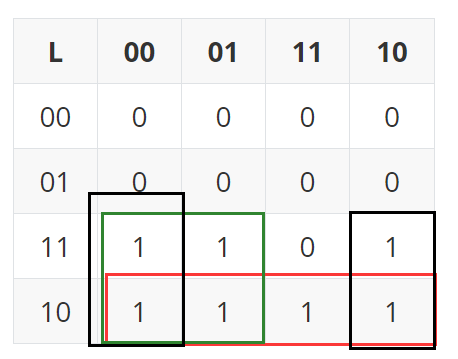
\includegraphics[scale=0.30]{SD2.4.3_1.png}
	\caption{2.4.3(1)}
\end{figure}
故原式$=A\overline{D}+A\overline{C}+A\overline{B}$\\
(2)先简单化简表达式:
$L=A\overline{B}CD+\overline{B}\cdot\overline{C}D+AB\overline{D}+BC\overline{D}+\overline{A}B\overline{C}$\\
卡诺图如下:(其中列为AB, 行为CD)
\begin{figure}[H] 
	\centering 
	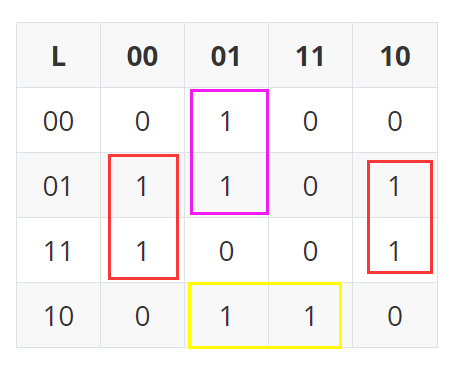
\includegraphics[scale=0.30]{SD2.4.3_2.png}
	\caption{2.4.3(2)}
\end{figure}
故原式$=B\overline{D}+\overline{A}\cdot\overline{C}D+A\overline{B}D$\\
(3)卡诺图如下:(其中列为AB, 行为CD)
\begin{figure}[H] 
	\centering 
	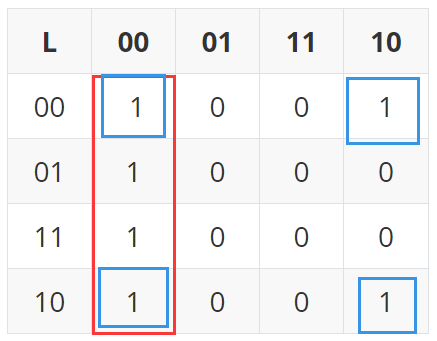
\includegraphics[scale=0.30]{SD2.4.3_3.png}
	\caption{2.4.3(3)}
\end{figure}
故原式$=\overline{C}\cdot\overline{D}+\overline{A}\cdot\overline{B}\cdot\overline{D}+AB\overline{D}$\\
(3)卡诺图如下:(其中列为AB, 行为CD)
\begin{figure}[H] 
	\centering 
	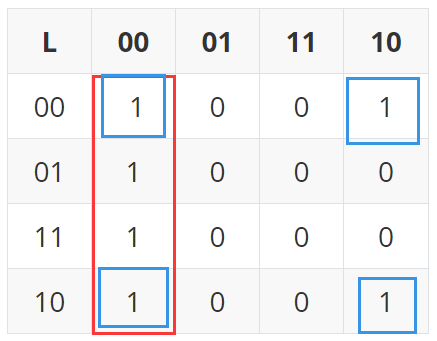
\includegraphics[scale=0.30]{SD2.4.3_3.png}
	\caption{2.4.3(3)}
\end{figure}
故原式$=\overline{C}\cdot\overline{D}+\overline{B}\cdot\overline{D}$\\
(4)卡诺图如下:(其中列为AB, 行为CD)
\begin{figure}[H] 
	\centering 
	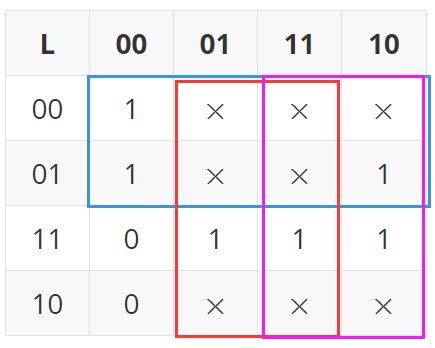
\includegraphics[scale=0.30]{SD2.4.3_4.png}
	\caption{2.4.3(4)}
\end{figure}
故原式$=\overline{A}+C+D$\\
\textbf{2.4.4} 用卡诺图化简法,求下列函数的最简或-与表达式\\
(1)$
L(A,B,C,D)=A\overline{C}+AD+\overline{B}\cdot\overline{C}+\overline{B}D
$\\
(2)$
L(A,B,C,D)=\sum m(3,4,5,7,13,14,15)
$\\
解:\\
(1)卡诺图如下:(其中列为AB, 行为CD)
\begin{figure}[H] 
	\centering 
	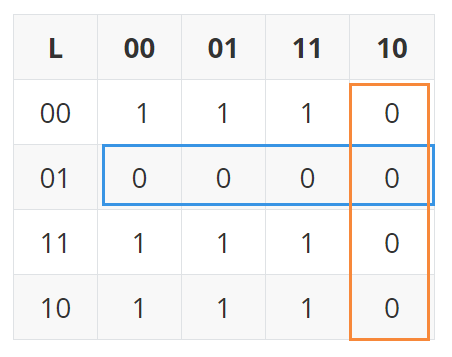
\includegraphics[scale=0.30]{SD2.4.4_1.png}
	\caption{2.4.4(1)}
\end{figure}
$\overline{L}=\overline{A}B+C\overline{D}\Rightarrow L=\overline{\overline{A}B+C\overline{D}}=(A+\overline{B})(\overline{C}+D)$\\
(2)卡诺图如下:(其中列为AB, 行为CD)
\begin{figure}[H] 
	\centering 
	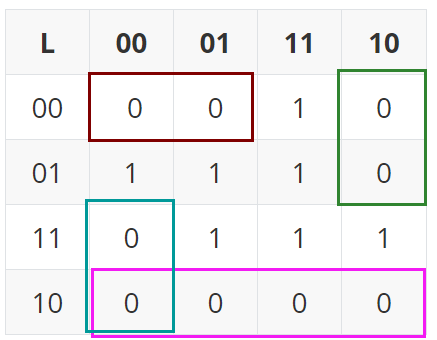
\includegraphics[scale=0.30]{SD2.4.4_2.png}
	\caption{2.4.4(2)}
\end{figure}
\noindent$\overline{L}=A\overline{B}+A\cdot\overline{C}\cdot\overline{D}+\overline{A}\cdot\overline{B}\cdot\overline{C}+\overline{A}C\cdot\overline{D}\\\Rightarrow L=\overline{A\overline{B}+A\cdot\overline{C}\cdot\overline{D}+\overline{A}\cdot\overline{B}\cdot\overline{C}+\overline{A}C\cdot\overline{D}}=(\overline{A}+B)(\overline{A}+C+D)(A+B+C)(A+\overline{C}+D)$





\end{document}